\subsection{Dispositivo}

El prototipo, al conectarse a una red eléctrica iniciará será el que inicie el asistente, al igual que dejará corriendo en segundo plano el subproyecto que hemos desarrollado con el fin de poder controlar y monitorizar el propio dispositivo.

    \subsubsection{Naturaleza del controlador}
    
        El monitoreo y control remoto de un dispositivo plantea el siguiente dilema: cómo invertir los roles para que un cliente haga de servidor recibiendo información, mientras el servidor hace de cliente mandando a este peticiones.
        
        Para resolver esta adversidad se toma una visión general del proyecto:
        \begin{enumerate}
            \item El dispositivo informa cada cierto tiempo de que sigue encendido.
            \item El servidor proporciona una API REST.
        \end{enumerate}
        
        Como bien se sabe, los operaciones básicas de una API REST son \textit{GET, POST, PUT y DELETE}, de modo que si se hace una petición \textit{GET} para informar sobre su conexión activa a la red eléctrica, se puede aprovechar por parte del servidor esta llamada para meter un mensaje específico en el cuerpo de la respuesta: este mensaje específico será el que propicie que se realice una acción en el dispositivo.
        
        De este modo el servidor podría manejar el dispositivo, monitorizándolo o pidiendo que haga acciones de manera remota, pudiendo tratarse por ejemplo de una tarea cuya finalidad sea que el asistente inicie una conversación con el usuario final en caso de que haya habido un accidente, de manera que se le pueda ayudar.
        
        Este planteamiento en cuanto a la naturaleza del controlador y su modo de uso parece factible, pero tiene la pega de la usabilidad, ya que si el dispositivo tiene una configuración de mandar su estado cada 24 horas, el control del dispositivo se demoraría demasiado, y aquí entra en juego la siguiente técnica:
        
        Se puede configurar en el propio dispositivo que las 24 horas que pasa entre aviso y aviso se obtengan a partir de un fichero de configuración, que permita la variación de estas 24 horas.
        También, en segundo plano, se puede configurar que a ciertas horas, el dispositivo disminuya su periodo de aviso, coincidiendo con unas ciertas horas relativas al horario de la jornada laboral del admnistrador del sistema, de modo que este pueda mandarle una primera tarea que sea otra reducción del periodo de aviso, por ejemplo a 10 segundos, permitiendo una comunicación síncrona más pareja a una comunicación real, y permitiendo un envío posterior de tareas al dispositivo que se realizarían en un espectro corto de tiempo.
        
        En la figura \ref{fig:prototype-flow} se puede observar el flujo de estados propuesto e implementado en este proyecto con el fin de poder controlar y monitorizar el dispositivo.
        
        \begin{figure}[h!]
            \centering
            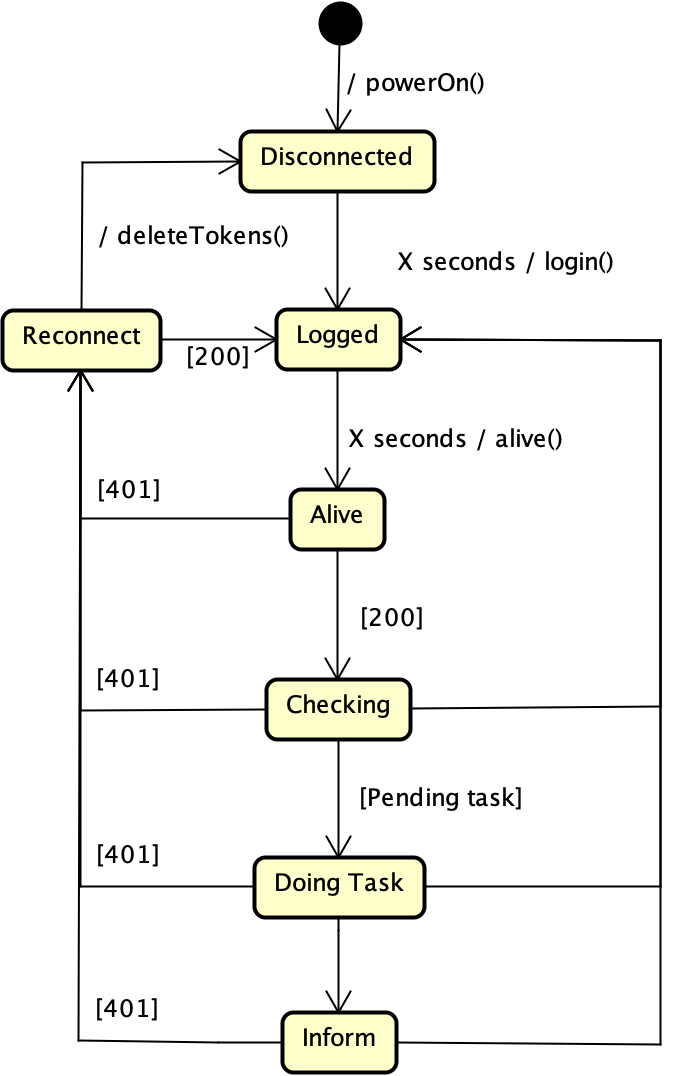
\includegraphics[width=7cm]{./img/state/prototype-flow.png}
            \caption{Flujo de estados del dispositivo}
            \label{fig:prototype-flow}
        \end{figure}
    
    \subsubsection{Desarrollo}
        Una vez planteada al teoría de cómo debe funcionar el asistente, toca ponerse con la práctica y demostrar que se puede formar un sistema que funcione y sea escalable.
        
        Para ello, se establece un espacio de trabajo dentro del dispositivo, el cual se vincula con un proyecto alojado en un servicio de control de versiones.
        De esta manera, se permite la posibilidad de actualizar las acciones del dispositivo con tan solo realizar una acción \textit{pull} del repositorio de origen.
        
        %% Sistema de arranque
        \textit{\textbf{Sistema de arranque}}
        
        El sistema implementado se ejecutará en el momento en el que se ejecute la clase \textit{Main.py}, que intenta iniciar sesión con el servidor a través del método \textit{signin()} de un objeto obtenido a través de la clase \textit{Login.py}.
        En el momento de instanciación del objeto \textit{login}, su constructor obtiene la dirección MAC del dispositivo, almacenándola en: 
        \begin{center}
        \textit{./cache/macfile.txt}
        \end{center}
        
        Esta dirección MAC propia y única para cada dispositivo, será utilizada como identificador en los credenciales a la hora de identificarse contra el servidor.
        La contraseña, será una encriptación de la dirección MAC que se obtiene simultáneamente en el constructor.
        
        Si se consigue iniciar sesión, se almacenan los tokens tanto en el objeto instanciado, como en el siguiente fichero externo:
        \begin{center}
        \textit{./cache/tokens.json}
        \end{center}
        
        Este almacenamiento externo permite su utilización a futuros programas que requieran los tokens para realizar peticiones contra el servidor. Continuando con el método el cual inició sesión, este devuelve un booleano, \textit{true}, desbloqueando un semáforo del \textit{main} que permite el envío al servidor del estado actual del dispositivo, a través de un método perteneciente a un objeto de tipo \textit{Alive.py}, el cual devuelve también otro booleano, que será \textit{false} en caso de que no se lleve la acción correctamente a cabo, cerrando el semáforo.
        
        Tras la implementación de este flujo de estados se ha podido comprobar la perfecta sincronía con el servidor, permitiendo proceder al diseño de un sistema que acepte la implementación de tareas.
        
        %% sistema de tareas
        \textit{\textbf{Sistema de tareas}}
        
        En el momento en el cual se hace la petición de \textit{/alive}, existen tres posibles respuestas por parte del servidor:
        \begin{enumerate}
            \item \textit{HTTP Status Code 200}: indica que la petición ha sido correcta.
            \item \textit{HTTP Status Code 300}: indica que la petición ha sido correcta, pero que hay múltiples respuestas, indicando al sistema del dispositivo que debe extraer la información que contiene el mensaje. En este mensaje, se incluye una lista de tareas pendientes del dispositivo:
            
        \begin{lstlisting}
        [{
            "id" : "task identifier",
            "device" : "device identifier",
            "event" : "TAREA",
            "by" : "who ordered this",
            "at" : "when it was ordered"
        }]
        \end{lstlisting}
        
        
            \item \textit{HTTP Status Code 401}: indica que el token ha dejado de ser válido, por lo que se debería volver a iniciar sesión, o refrescar el token. Como un token de acceso tiene establecido por razones de seguridad un tiempo de validez de 30 minutos, y el dispositivo en principio realizará la petición de mostrar que sigue activo cada 24 horas, no se ve necesaria la implementación en el dispositivo de un método que refresque el token, ya que produciría un aumento del consumo de datos, al refrescar constantemente un token al que no va dar uso.
            
        \end{enumerate}
        \label{seq:received300}
        
        Una vez recibida una respuesta de tipo \textit{HTTP Status Code 300}, se procede a analizar las tareas pendientes que están en el cuerpo del mensaje. Para ello, se procede a ejecutar siempre la primera de la lista gracias a que han sido devueltas por orden de asignación desde el servidor.
        Analizando los campos de la tarea, vemos que dispone de campo llamado \textbf{event}, el cual indica el nombre de la tarea a realizar.
        
        El nombre de la tarea es único, y debe ser una palabra sin espacios, permitiendo utilizarlo como palabra clave.
        Gracias a esta palabra clave, se puede pedir al dispositivo que ejecute la tarea concreta, y para ello administramos el sistema de ficheros de modo que siga la siguiente estructura:
        
        \begin{center}
            \textit{./task/TAREA/}
        \end{center}
        y dentro de ese directorio, debe haber un script, el cual ejecute la tarea específica:
        
        \begin{center}
            \textit{./task/TAREA/init.sh}
        \end{center}
        
        \begin{figure}[h!]
            \centering
            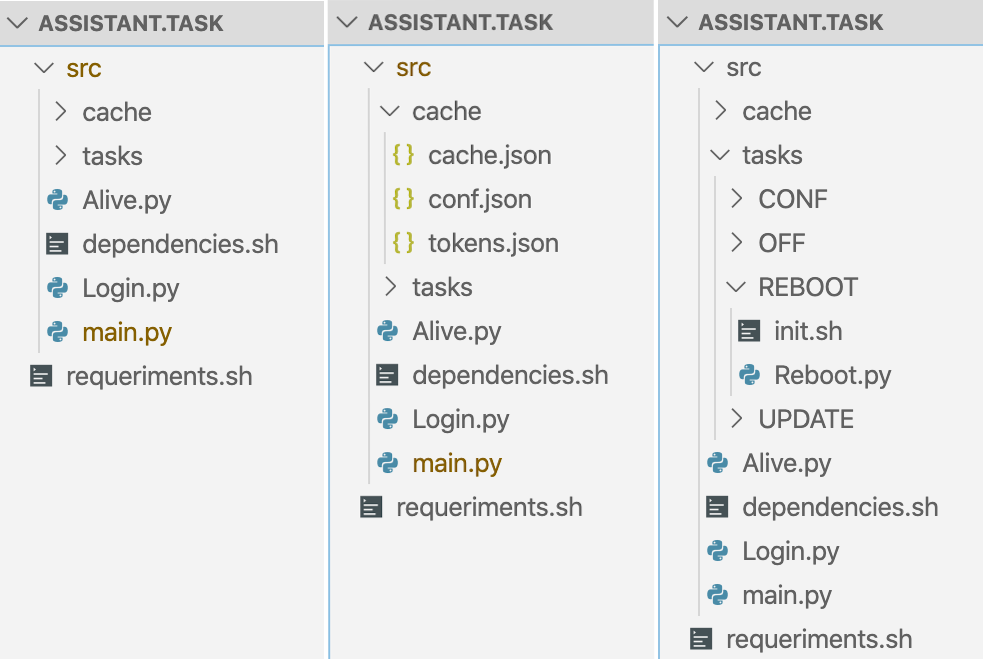
\includegraphics[width=10cm]{./img/arch/device/src.task.png}
            \caption{Contenido global del repositorio}
            \label{fig:src.task}
        \end{figure}
        
        Este script, puede llamar a otros programas o a otros scripts, de modo que se permite la realización de cualquier evento configurado.
        
        Una vez se tiene esta estructura implementada, como se puede observar en la figura \ref{fig:src.task}, tan solo hay configurar que al recibir como respuesta del servidor un código 300, se ejecute el script que está almacenado en la dirección obtenida al sustituir el nombre de la tarea, por ejemplo, \textbf{REBOOT}, en la ruta base:
        
        \begin{lstlisting}
            sh ./task/REBOOT/init.sh
        \end{lstlisting}
        
        Como se puede observar, este método de organización de tareas posibilita la fácil implementación de nuevas tareas sin poner en peligro las ya creadas, ya que únicamente se necesita crear un directorio nuevo por cada nueva tarea, y un script que inicie las acciones a realizar.
        
        %% estructura global
        
        
        
        %% inicio automático
        \textit{\textbf{Inicio automático}}
        
        Ya se tiene una configuración válida para el dispositivo, pero hay que poder asegurar su buen despliegue e inicio al reiniciar el dispositivo, de modo que se pueda tener como un valor seguro que, si un usuario reinicia la máquina físicamente, este dispositivo será capaz de iniciar el sistema ahora creado para poder monitorizarlo y controlarlo.
        
        Entonces, para la configuración del espacio de trabajo se proporciona un script que permite la configuración del dispositivo en caso de ser la primera vez que se utiliza ese dispositivo, por si no se han cargado bien los servicios.
        
        En dicho script, almacenado como \textit{requirements.sh}, se establecen dos pasos claves del proyecto:
        
        \begin{enumerate}
            \item La configuración para el inicio automático del sistema de control remoto del dispositivo a través de la herramienta de \textit{crontab} que proporcionan los sistemas Unix.
            
        \begin{lstlisting}
        # configure scheduled task
        (crontab -l ; echo "@reboot sleep 60; cd /home/pi/assistant.task/src/ ; python /home/pi/assistant.task/src/assistant-alive.py & > home/pi/assistant.task/src/cache/logfile.txt") | crontab -
        \end{lstlisting}
        
        De este modo, se abre el fichero de configuración de \textit{crontab} en el cual se plasma qué es lo que se desea que se ejecute en cada reinicio, como indica la etiqueta \textit{@reboot}.
        Si se presta atención al script, se solicita una espera de 60 segundos a partir del reinicio del dispositivo, y el motivo por el cual se establece ese tiempo es para permitir que el dispositivo pueda configurar su conexión a internet y levantar previamente todos sus servicios antes de que el sistema aquí descrito arranque, evitando posibles interferencias que no permitiese arrancar de la manera correcta, como puede ser una mala obtención de la dirección MAC de la tarjeta de red.
        
        \item El script de lo requisitos ejecuta otro script, el de la instalación de las dependencias, el cual permite la instalación de las librerías de python requeridas para el correcto funcionamiento del dispositivo.
        
        \begin{lstlisting}
        # install python dependencies
        sudo sh ./src/dependencies.sh
        \end{lstlisting}
        
        De esta manera, se establecen las medidas y acciones necesarias, al igual que los scripts requeridos para poder asegurar el cumplimiento y buen funcionamiento del dispositivo aplicando los protocolos de comunicación descritos.
        
        \end{enumerate}


\subsection{BackEnd}

    \subsubsection{Introducción}

        Para el desarrollo del BackEnd se va a seguir la arquitectura descrita en el apartado \ref{arch-be}, de modo que a continuación se describirá cómo esa arquitectura ha sido implementada, con qué herramientas, y cuáles son las dependencias o servicios que posee.

    \subsubsection{Principios de diseño}
    
        Para un buen desarrollo de un sistema software se debe seguir los patrones de diseño, al igual que se deben aplicar los diferentes principios de diseño.
        
        A la hora del desarrollo, se ha considerado respetar los principios de diseño \textbf{SOLID}~\cite{clean-arch-book}:
        
        \begin{enumerate}
            \item Open-Closed Principle:
            
            Partimos de un lenguaje como Kotlin el cual toda clase de datos es cerrada en cuanto a extensión. De este modo, se ha asegurado que toda clase que se requiera como abierta lleva el operador \textit{open} con ella.
            
            \item Single responsability Principle:
            
            Se ha respetado que cada clase tenga únicamente una única función, dividiendo en varias toda clase que requiera más de una responsabilidad. Esto se ha podido asegurar a la hora de la implementación y segregación del sistema en servicios a la hora de acceder a la base de datos, al igual que en los múltiples controladores que posee el sistema con tal de acceder y realizar funciones diferentes.
            
            \item Liskov Substitution Principle:
            
            El principio de sustitución de Liskov nos dice que debemos perservar el funcionamiento de una interfaz o clase en el momento que la heredamos, de modo que una redefinición de un método debe poder cumplir los contratos. Este principio se ha complido a la hora de implementar los servicios, ya que se ha requerido que cumplan todos y cada uno de los requisitos impuestos en las interfaces de la capa de la lógica del sistema.
            
            \item Dependency Inversor Principle:
            
            El sistema ha sido implementado siguiendo el esquema de The Clean Arquitecture, como ya se ha nombrado anteriormente, de modo que los endpoint de la API Rest son quienes solicitan a los controladores la realización de cierto caso de uso.
            Los controladores, para la realización de estos casos de uso pueden requerir el acceso a servicios o repositorios externos. Para ello, cada controlador indica cuales son los servicios que va a necesitar, y si un servicio quiere servir al caso de uso, debe cumplir con los contratos establecidos en la interfaz pública del caso de uso.
            De esta manera, siguiendo todos los principios anteriores, se cumple este principio ya que si el servicio integra la interfaz, el servicio puede ser inyectado en el caso de uso, permitiendo una estanquedad de los controladores a los servicios externos, y con ello facilitanto el cambio de un servicio por otro sin que afecte al sistema, y cumpliendo así el principio de inversión de dependencia.
            Para la inyección de estas dependencias ha sido utilizado el framework de Koin, el cual ha sido explicado anteriormente en el apartado \ref{Koin}.
            
            \item Interface Segregation Principle:
            
            El principio de segregación de interfaces nos indica que una buena práctica se basa en contar con varias interfaces específicas de modo que se pueda utilizar una u otra en función del tipo de cliente.
            Esto se ha llevado a cabo a la hora de comprobación de credenciales, ya que se proporciona una interfaz u otra en función de si el token recibido viene por parte de un dispositivo, o de un administrador, pudiendo ambos iniciar sesión, pero ejecutándolo diferentes controladores.
            
        \end{enumerate}
        
        En cuanto a patrones de diseño, se han seguido en mayor medida los descritos a continuación gracias a haber aplicado los principios SOLID descritos anteriormente:
        
        La elaboración de un sistema por capas con una comunicación de dependencias lineal nos permite la utilización del \textbf{patrón fachada}, ya que para la conexión entre servicios y controladores hay una interfaz pública la cual limita el número y tipo de objetos que se mandan entre ambos, evitando una sobrecomunicación, al igual que una relación de dependencias circulares.
        
        Gracias a la aplicación de este patrón, se da cabida a la posibilidad de aplicación del \textbf{patrón adaptador}, permitiendo la creación de unas nuevas interfaces intermedias que adapten las interfaces públicas de los controladores a posibles futuros servicios que sustituyan a los actuales, sin necesidad de modificar el comportamiento de los controladores los cuales ya realizan los casos de uso, y asegurando entonces un aislamiento escalable.
        
        También, los servicios han servido de punto de acceso a la información de la base de datos gracias al uso del framework \textit{ExposedSQL}, de modo que ha intercambiado la información con los controladores a través de objetos, separando por tanto el acceso a la BBDD de la capa de negocio, aplicando por tanto el \textbf{patrón DAO} y posibilitando cambiar en un futuro el sistema de almacenaje de información sin que requiera un solo cambio en la capa de negocio del sistema.
        
        A la hora de mantener un registro de cómo está funcionando el sistema, se ha utilizado el \textbf{patrón Singleton} con el fin de obtener una instancia del objeto Logger, y con ello poder retransmitir logs desde cualquier punto del sistema sin requerir aumentar los recursos y evitando errores de interferencias por re-declaración. También, se ha aplicado este patrón para el acceso al \textit{TokenStore}, el cual almacena los tokens activos, y de esta manera permitir la comunicación entre el controlador de sesión con el servidor OAuth a través de la misma instancia, ya que al instanciar un nuevo objeto se perderían los tokens activos ya creados.
    
    \subsubsection{Servicios}
    
        Los servicios forman el acceso a la capa más externa según el esquema de \textit{The Clean Architecture}, y han sido implementados aceptando y cumpliendo las condiciones impuestas en las interfaces públicas de la capa de negocio.
        
        De esta manera, los servicios que requiere el sistema son los siguientes:
        \begin{enumerate}
            \item\textit{ConfService:}
            A través de este servicio se puede obtener cualquier configuración existente, ya sea de los dispositivos, de las localidades, o globales. También tiene la opción de marcar ciertas configuraciones como ya instaladas, crear nuevas, o borrarlas en función del identificador o de su estado.
            
            \item\textit{DeviceService:}
            Este servicio proporciona la información relativa a un dispositivo, siendo posible comprobar si un dispositivo existe en el sistema, comprobar las credenciales, crear uno nuevo, obtener todos, obtener el dispositivo asociado a un determinado usuario, asignar un dispositivo a un usuario concreto, o almacenar y recolectar los últimos estados del dispositivo.
            
            En este servicio se puede apreciar la utilidad de segregar el sistema en servicios, al igual que la inversión de dependencias, ya que se podría sustituir facilmente el servicio cambiando por tanto la manera en la que se registran los dispositivos, o cambiando la manera en la que se comprueban las credenciales, que en el caso de este sistema es mediante la encriptación de la dirección MAC, por otro tipo de comprobación sin alterar el funcionamiento de la capa de negocio, que seguiría aislada.
            
            \item\textit{IntentsService:}
            Permite almacenar las actividades realizadas en los dispositivos, es decir, la información relevante obtenida tras una comunicación \textit{máquina-usuario}. También permite obtenerlos, ya sea el último de una máquina, o una lista de los realizados por un dispositivo específico entre dos fechas.
            
            \item\textit{LocationService:}
            Ofrece la posibilidad de almacenar nueva localidades y luego recopilarlas ya sean todas, por código postal, o por provinicias.
            
            \item\textit{PeopleService}
            Relativo a los clientes que tendrán en su poder un dispositivo. Es útil para añadir personas y para obtenerlas después ya sean todas, o por su nif, o por código postal, al igual que poder obtener los datos sobre el dispositivo asignado para una persona en concreto.
            
            \item\textit{TaskService:} Controla la información almacenada sobre los eventos y tareas asignadas a dispositivos, de manera que permite la adición y obtención de eventos, al igual que de dispositivos. También permite la obtención de tareas pendientes de un dispositivo concreto, o la recolección de todas las tareas de un dispositivo concreto ocurridas en un rango de tiempo concreto.
            
            \item\textit{UserService:} Este servicio lleva la gestión de usuarios del sistema, es decir, de administradores del sistema, que son diferentes que los clientes de los dispositivos. Estos usuarios poseen una contraseña y el servicio ofrece la manera de verificar que sus credenciales son correctos.
            
        \end{enumerate}
    \subsubsection{Más a fondo}
    
    Debido a la complejidad del sistema, se ilustrará el diseño del sistema con varias figuras y sus explicaciones correspondientes con el fin de que el lector pueda comprender la implementación y replicarla en un futuro, al igual que pueda modificar lo que requiera, si en un futuro quiere tomar este documento como manual para una reimplementación del sistema.
    
    El backend estará estructurado en 3 capas:
    
    \begin{figure}[H]
    \centering
        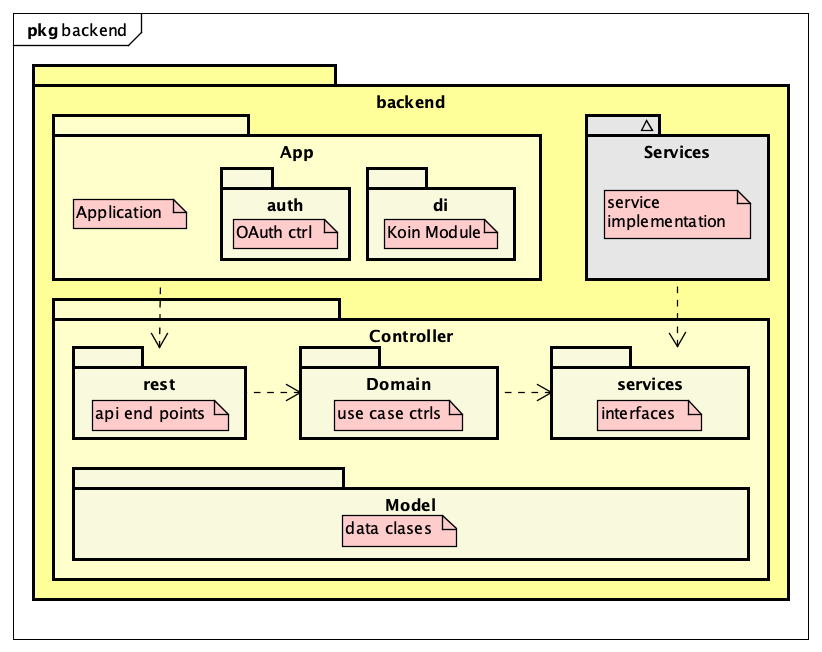
\includegraphics[width=10cm]{./img/arch/back/diagram.design.png}
        \caption{Diagrama de diseño}
        \label{fig:designdiagram}
    \end{figure}

    \begin{enumerate}
        \item \textbf{App:}
        Albergará la aplicación que iniciará el sistema, al igual que tendrá dos subdirectorios. El directorio \textit{auth} manejará la configuración sobre los tokens de acceso, y el directorio \textit{di} será el que contenga la configuración del inyector de dependencias, el cual se configura mediante la implementación de un módulo.
        
        \item \textbf{Controller:}
        Se asocia a la \textit{capa de negocio} del sistema, de modo que se puede considerar el componente aislado principal del sistema, ya que no depende de ninguna clase externa y proporciona modos mediante los cuales se puede acceder a su uso.
        Internamente, se puede observar el directorio \textit{rest}, el cual contiene los end-points del sistema, los cuales se explicarán más adelante. Otro de los directorios es el subdirectorio de \textit{Domain}, el cual contiene los controladores mediante los cuales se realizan los casos de uso. Estos controladores tienen la lógica del sistema, y para acceder a recursos externos como puede ser la base de datos u otros servicios externos, utilizan servicios externos inyectados a través del framework, siempre y cuando esos servicios externos utilicen las interfaces que proporcionan los controladores. El tercer directorio es el de \textit{services}, el cual contiene las interfaces requeridas por los controladores y consiguiendo con esto una inversión de dependencias, ya que de requerir un servicio por parte del controlador, se ha pasado a que el servicio requiera, para poder ser utilizado, la implementación de estas interfaces.
        
        Se puede observar un cuarto directorio, \textit{Model}, el cual contiene clases que serán utilizadas para el envío de datos entre las diferentes capas, evitando la utilización en esta capa de negocio de clases de datos externas que produzcan una dependencia.
        
        \item \textbf{Services:}
        Son los servicios externos que proporcionan información al sistema. Estos servicios deben implementar las interfaces de servicios que proporciona la capa de negocio. De este modo, si las implementan, pueden ser inyectados a través del inyector de dependencias.
    \end{enumerate}
    


    La aplicación que arranca el sistema y maneja toda la configuración es \textit{./src/app/Application.kt}.
    
    En cuanto a los endpoints del sistema, se pueden declarar en la propia aplicación, pero se considera buena-práctica el disgregarlos en diferentes módulos, agrupados por rutas o servicios similares, obteniendo así una mejor visibilidad y permitiendo un acceso intuitivo a la hora del desarrollo.
    
    A cada módulo de ruta se le otorga el acceso a los servicios necesarios que va a requerir los controladores. De este modo, al declarar los end-points se le proporcionan los servicios en su constructor, y se evita una dependencia directa de la capa de negocio con el framework elegido para inyectar esas dependencias, ya que las dependencias se inyectan en el módulo iniciador de la aplicación, el cual es externo a la capa de negocio, siguiendo manteniéndola aislada del exterior.
    
    En el siguiente diagrama se puede observar los 3 subpaquetes ya descritos anteriormente que conforman el sistema, al igual que las dependencias entre ellos: tanto el paquete \textit{App} como el paquete \textit{Services} dependen del paquete \textit{Controller}, el cual no depende de ningun otro y por tanto, está aislado de los cambios del exterior.
    
    \begin{figure}[H]
    \centering
    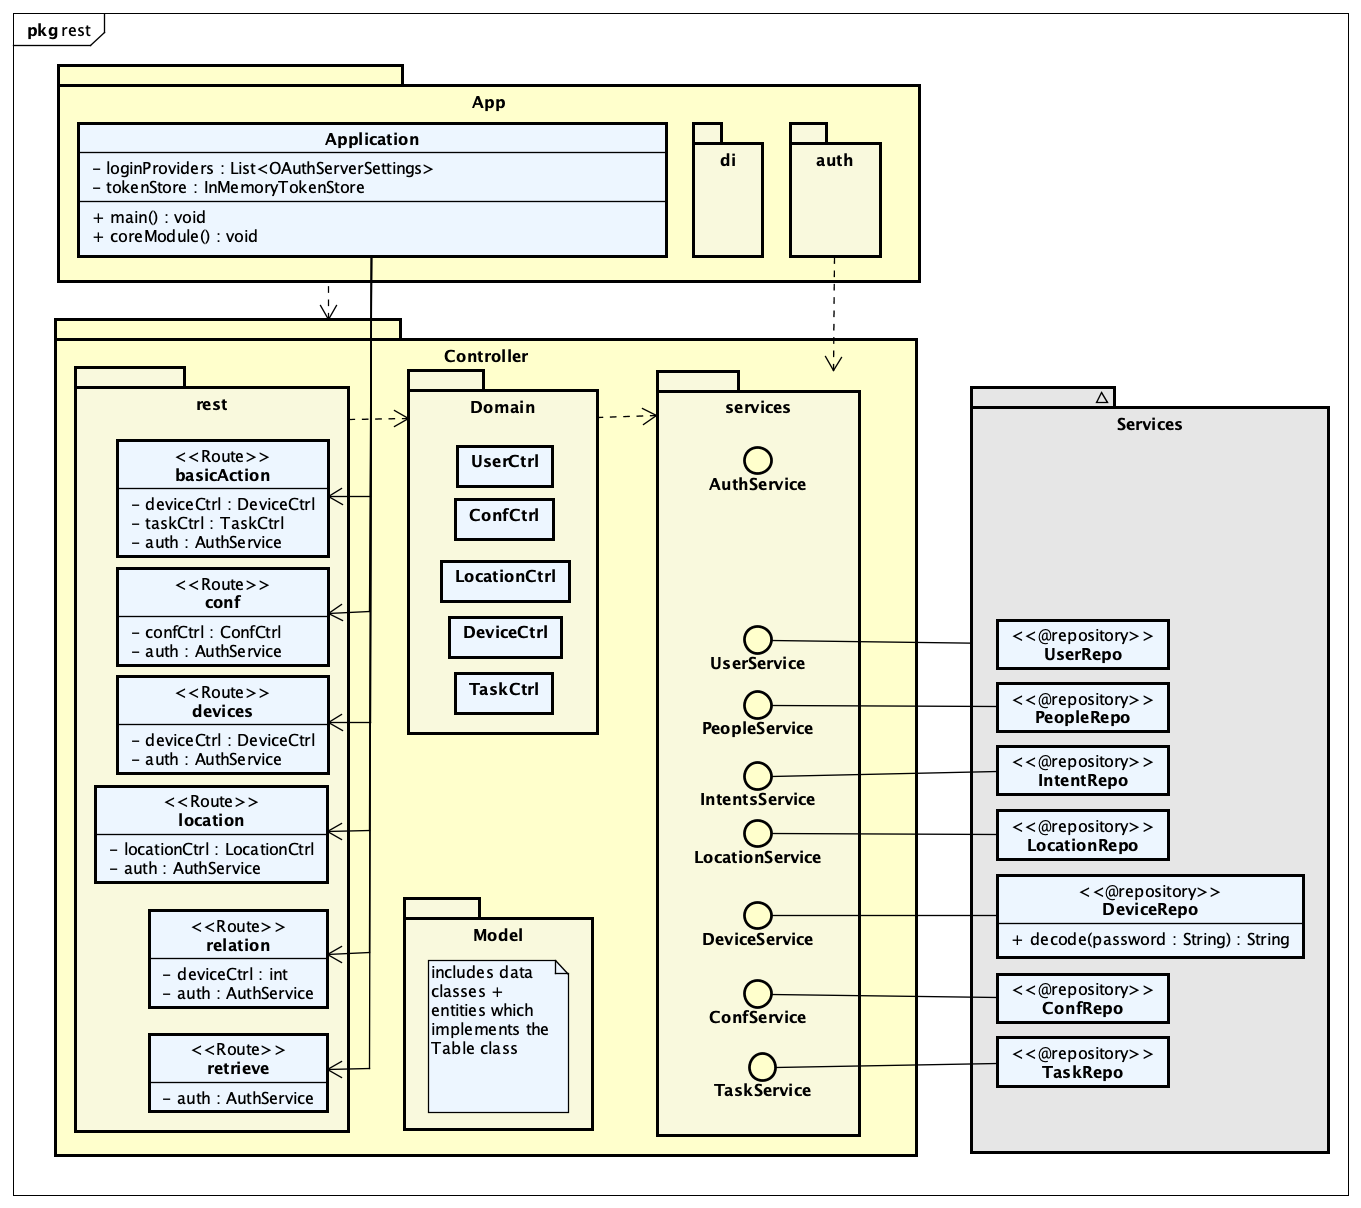
\includegraphics[width=14cm]{./img/arch/back/diag.class.2.png}
    \caption{Diagrama de Clases: General}
    \label{fig:diagram.app}
\end{figure}

    En la figura anterior se ha podido ver la estructura y dependencias de cada subpaquete de manera general.
    Ahora, se particularizará mostrando la estructura interna de cada uno de ellos, explicándo qué es y para qué se utiliza cada parte.
    
    Teniendo en cuenta la figura \ref{fig:dc.app}, podemos observar diferentes partes:
    
    Por un lado, tanto \textit{InMemoryIdentityCustom} como  \textit{InMemoryTokenStore}, que son modificaciones del framework OAuth que permiten la utilización del store de tokens fuera del framework, de modo que los tokens se puedan gestionar a través del sistema. Su instalación ya ha sido explicada en el apartado \ref{oauth20}, de modo que no se va a entrar ahora de nuevo.
    
    Una vez ya obtenido un acceso público de \textit{TokenStore}, este será gestionado únicamente desde el servicio creado para el control de tokens, \textit{TokenCtrl}, el cual implementa la interfaz \textit{AuthService}, permitiendo que este servicio sea inyectado en el sistema.
    
    Esta inyección se produce tras la implementación en \textit{Application} del módulo de dependencias creado con Koin, \textit{app.di.Module.myModule}, el cual también ha sido explicado cómo debe ser instalado en la aplicación en el apartado \ref{Koin}, al igual que el resto de servicios.
    
    La aplicación, por tanto, obtendrá los servicios inyectados y se los proporcionará a cada ruta, como se pueden observar en la figura \ref{fig:dc.app}, de modo que la capa de negocio ya dispondrá de los servicios para su uso, a través de las interfaces que había predefinido.

    \begin{figure}[H]
        \centering
        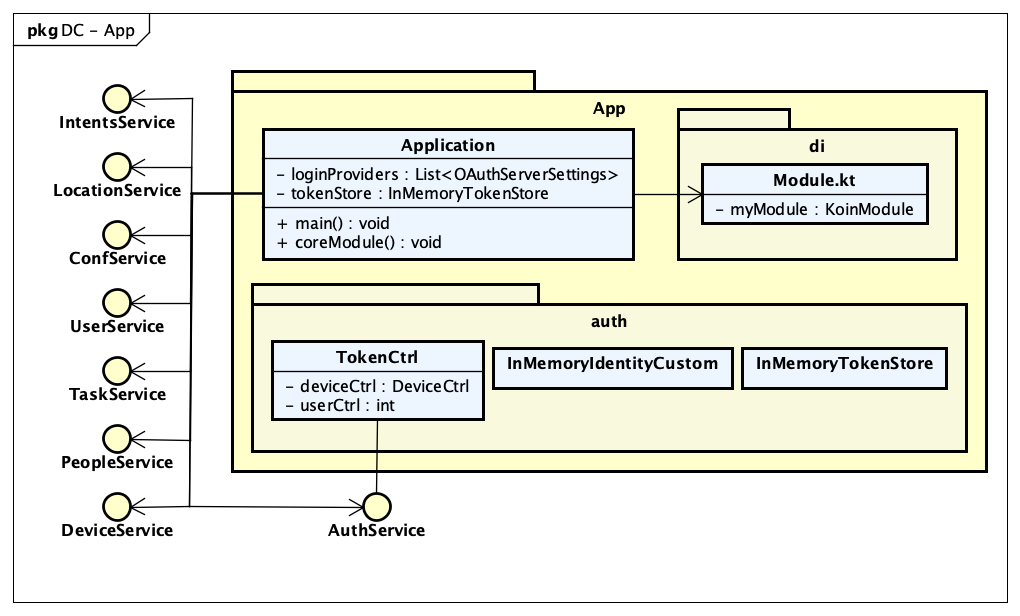
\includegraphics[width=14cm]{./img/arch/back/dc.app.png}
        \caption{Diagrama de Clases: App}
        \label{fig:dc.app}
    \end{figure}

    En cuanto a la capa de negocio expuesta en la \ref{fig:diagram.app} como \textit{Controller}, se puede observar que los paquetes \textit{Domain}, \textit{services}, y \textit{Model} no han sido explicados, por lo que se mostrará en las siguientes figuras su contenido.
    
    Se puede observar en la figura \ref{fig:dc.domain} que \textit{Domain} contiene el dominio de la aplicación, gestionando los controladores que hacen que se cumplan todos los casos de uso descritos anteriormente, almacenando toda la lógica del sistema.
    
    Cada controlador tiene atribuídas unas las dependencias, que están relacionadas con las interfaces descritas por esta capa de negocio, asegurando por tanto que no se va a tener que implementar ninguna operación externa.

    Las interfaces \textit{-descritas en la figura \ref{fig:dc.services}-} muestran las operaciones requeridas por los controladores, sirviendo de contrato para los servicios externos que quieran dar un uso futuro al sistema.
    
    \begin{figure}[H]
        \centering
        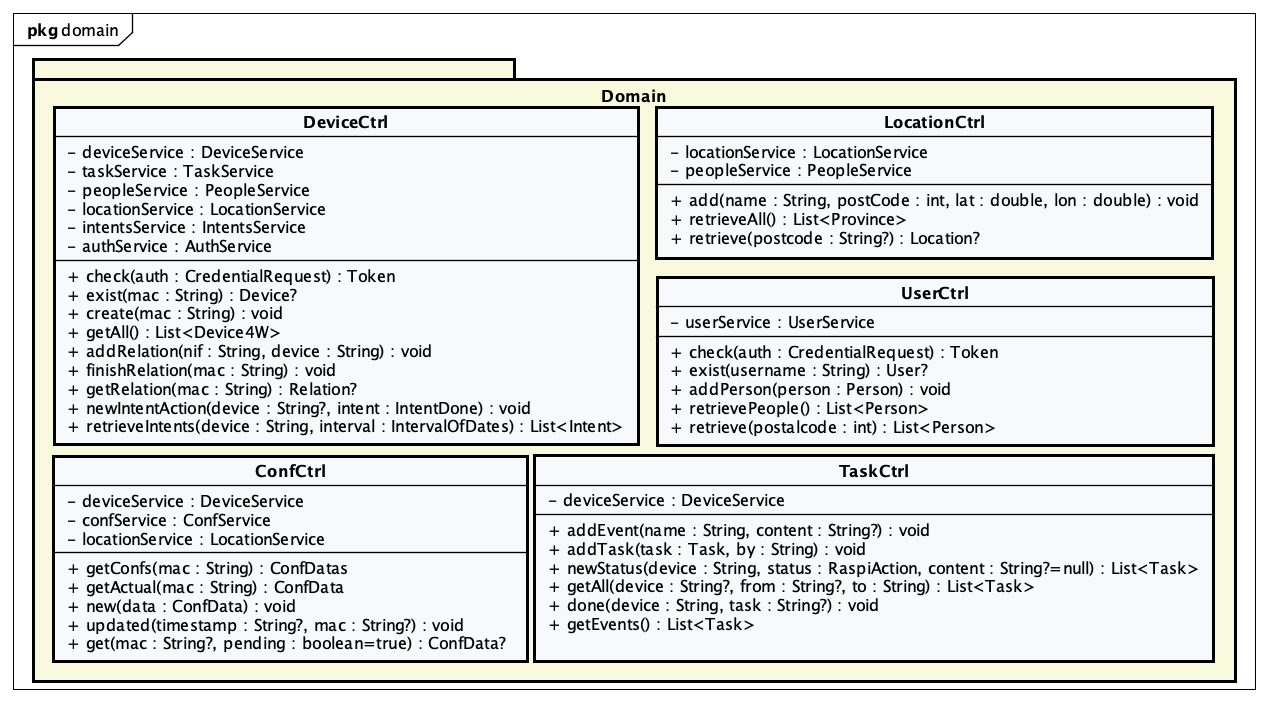
\includegraphics[width=13cm]{./img/arch/back/dc.domain.png}
        \caption{Diagrama de Clases: Domain}
        \label{fig:dc.domain}
    \end{figure}
        
    \begin{figure}[H]
        \centering
        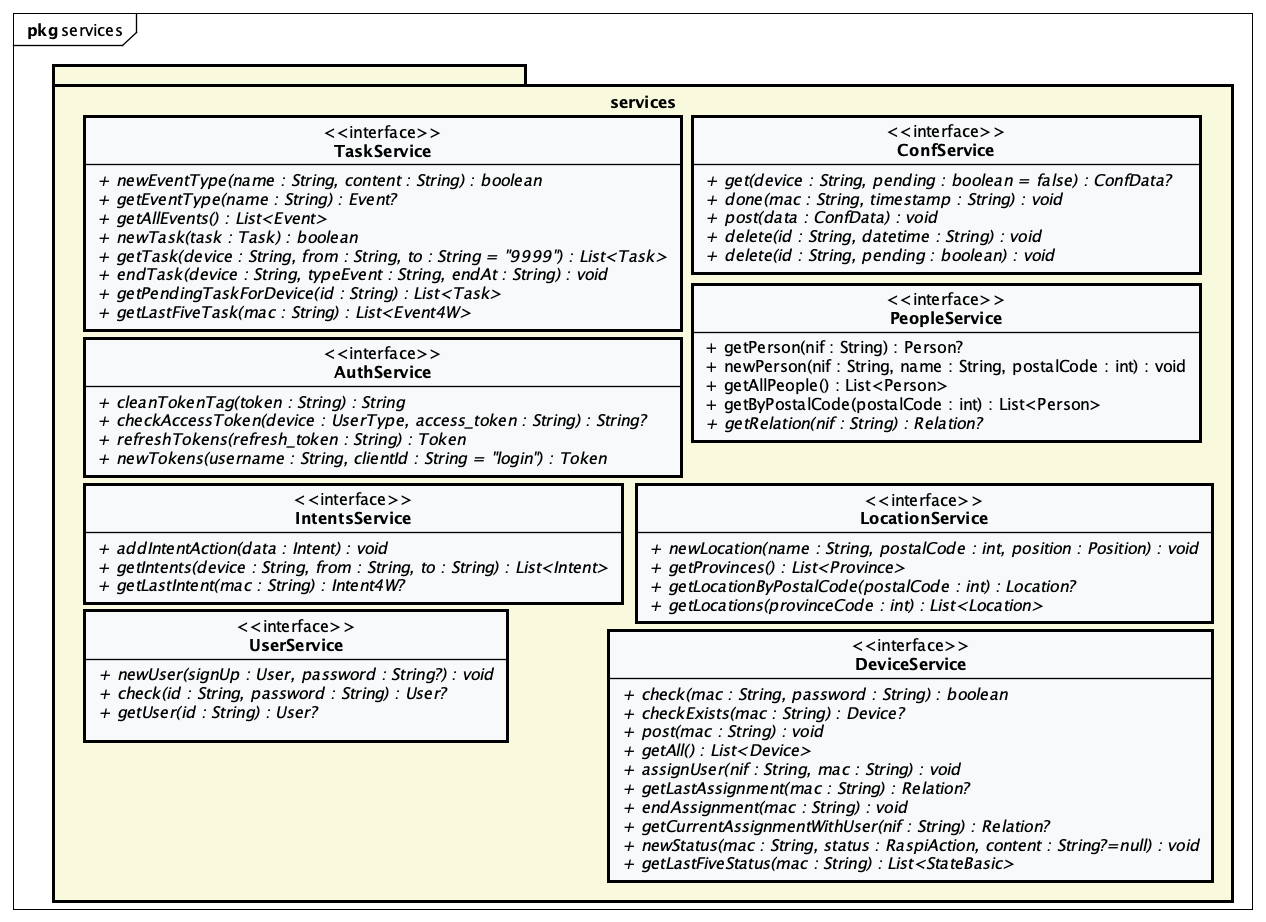
\includegraphics[width=14cm]{./img/arch/back/dc.services.png}
        \caption{Diagrama de Clases: Services}
        \label{fig:dc.services}
    \end{figure}

    Para la comunicación entre la capa de negocio con las otras capas, al igual que para la gestión de la información en comunicaciones internas se necesitan unas clases que sirvan para el envío de datos, favorenciendo y simplificando la comunicación.
    
    Estas clases, llamadas \textit{clases de datos}, son las mostradas a continuación en la figura \ref{fig:dc.model}.

    \begin{figure}[H]
        \centering
        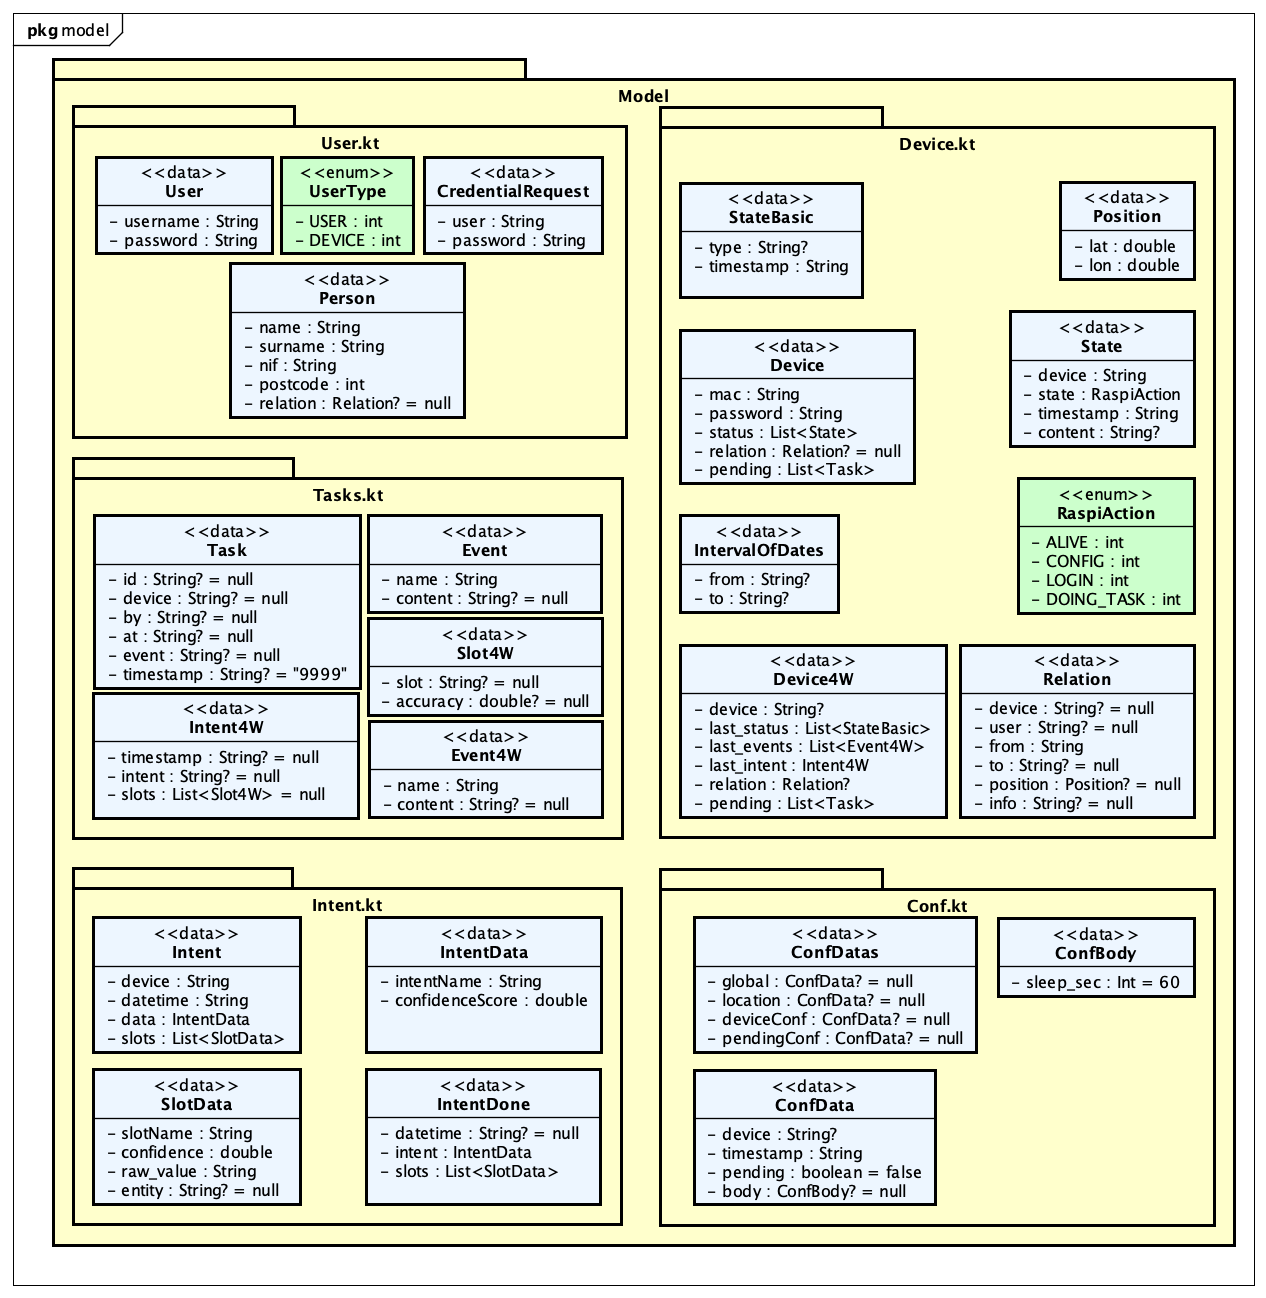
\includegraphics[width=14cm]{./img/arch/back/dc.model.png}
        \caption{Diagrama de Clases: Model}
        \label{fig:dc.model}
    \end{figure}


    \newpage
    \subsubsection{Diagrama Entidad-Relacion}
    
    En el siguiente diagrama, representado con la figura \ref{fig:d.er}, se puede observar cuales son las relaciones entre las distintas tablas que componen la base de datos, de modo que se aprecian las dependencias de claves que comparten entre si.
    
\begin{figure}[H]
    \centering
    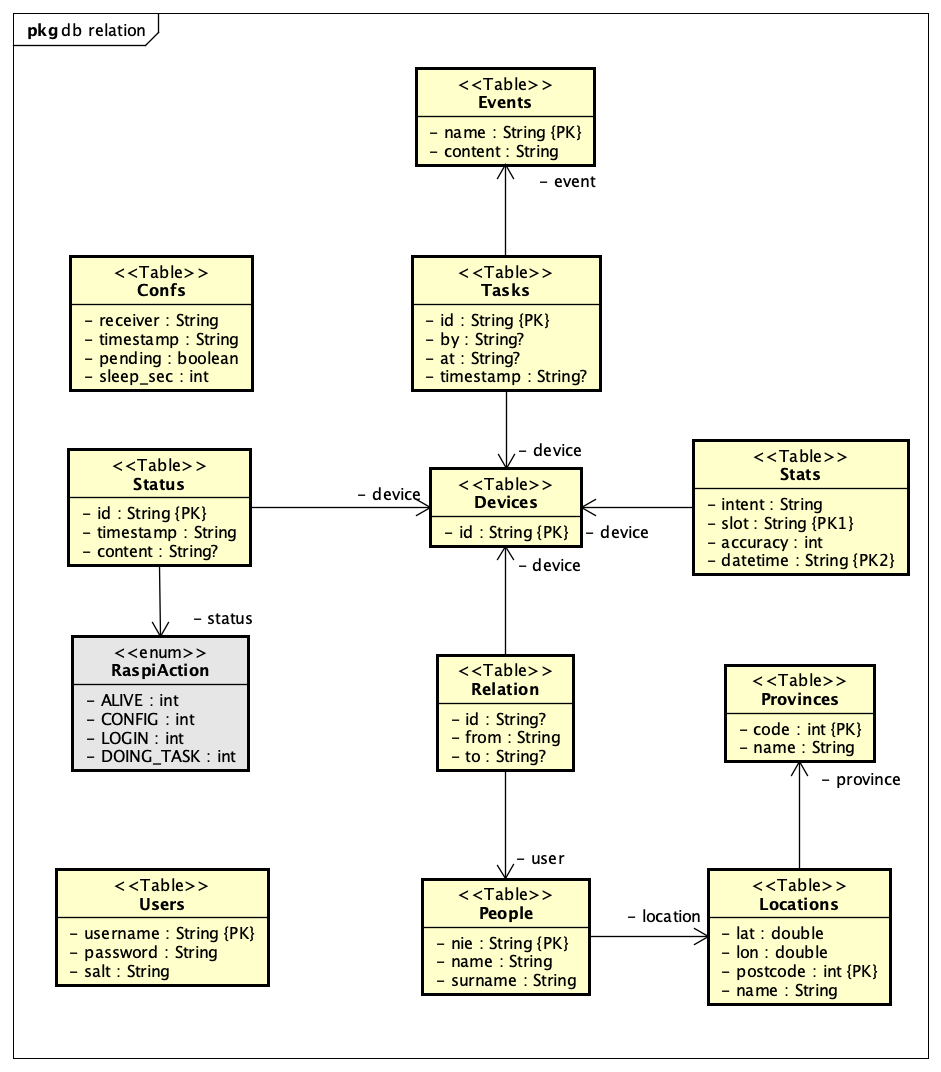
\includegraphics[width=14cm]{./img/arch/back/d.er.png}
    \caption{Diagrama Entidad-Relación}
    \label{fig:d.er}
\end{figure}

    \subsubsection{End-Points}
    Los end-points del sistema se van a diferenciar en dos tipos: los habilitados para el dispositivo, que comienzan por \textit{/device}, y los habilitados para el administrador , que comienzan por \textit{/worker}.

De esta manera, el sistema validará el token recibido en la petición, obteniendo qué tipo de usuario es, y sólo dejará acceder al recurso si el usuario es del tipo correcto para esa llamada.

Todas las llamadas, excepto las de inicio de sesión y de refresco de credenciales, deberán contener el token de acceso como parámetro del header.

En cuanto a las posibles respuestas para las llamadas, hay 3 respuestas prestablecidas:
\begin{enumerate}
    \item HttpStatusCode 401 : Unauthorized.\newline
    Se da cuando los credenciales introducidos en el inicio de sesión no son correctos, o cuando el token de acceso no sea válido, ya sea por haberse expirado, por ser falso o por ser de un tipo de usuario no permitido para esa llamada.
    
    \item Http Status Code 400 : Bad Request.\newline
    Se va a obtener cuando los datos introducidos en la llamada no son válidos, ya falte algún parámetro en el formulario, o no cumplan con las especificaciones.
    
    \item Http Status Code 500 : Internal Server Error.\newline
    Será devuelto cuando la llamada haya sido completamente correcta, pero el procesado de ella haya dado con algún tipo de error en el lado del servidor. En este caso, se deberá contactar con el administrador del BackEnd.
    
\end{enumerate}

%%%%
\textbf{[POST] \textit{/device/login }}
\textit{Inicio de sesión con un dispositivo.}

    Parámetros de la llamada:
    \begin{lstlisting}[language=json,firstnumber=1]
        "user" : "mac"
        "password" : "encrypted mac"
    \end{lstlisting}
    
    RESPONSE:\newline
        \textit{Http Status Code 200 : Ok}
        
    \begin{lstlisting}[language=json,firstnumber=1]
    {
        "access_token" : "Bearer lo-que-sea-de-acceso",
        "refresh_token" : "Bearer lo-que-sea-de-refresco"
    }
    \end{lstlisting}    
\newpage
%%%%
\textbf{[GET] \textit{/device/alive }}
\textit{Envío de ping de dispositivo.}
    
    RESPONSE:\newline
    \textit{Http Status Code 200 : Ok}
    
    \begin{lstlisting}[language=json,firstnumber=1]
    {"status": 200, "action": "ALIVE"}
    \end{lstlisting}
    \textit{Http Status Code 300 : Multiple Choices}
    
    \begin{lstlisting}[language=json,firstnumber=1]
    JSONarray<Task>
    \end{lstlisting}
\hline 
\newline
%%%%
\textbf{[GET] \textit{/device/tasks/:id/doing }}
\textit{Aviso de ir a realizar una tarea, especificando su identificador.}
    
    RESPONSE: \newline
    \textit{Http Status Code 200 : Ok}
    
    \begin{lstlisting}[language=json,firstnumber=1]
    {"status": 200, "action": "ALIVE"}
    \end{lstlisting}
\hline 
\newline
%%%%
\textbf{[GET] \textit{/device/confs }}
\textit{Devuelve la configuración más actual del dispositivo.}
    
    RESPONSE: \newline
    \textit{Http Status Code 200 : Ok}
    
    \begin{lstlisting}[language=json,firstnumber=1]
    JSON<ConfData>
    \end{lstlisting}
\hline 
\newline
%%%%
\textbf{[GET] \textit{/device/confs/:timestamp }}
\textit{Aviso del dispositivo de haber instalado la configuración que tiene un timestamp concreto.}

    RESPONSE: \newline
    \textit{Http Status Code 200 : Ok}
    
    \begin{lstlisting}[language=json,firstnumber=1]
    Configuration has been updated on device.
    \end{lstlisting}
\hline
%%%%
\textbf{[POST] \textit{/device/intents }}
\textit{Aviso del dispositivo de haber realizado una conversación con el usuario, enviando los datos básicos.}

    BODY:
    \begin{lstlisting}[language=json,firstnumber=1]
    JSON<IntentDone>
    \end{lstlisting}
    
    RESPONSE: \newline
    \textit{Http Status Code 200 : Ok}
    
\newpage %% NEW PAGE

Entre todas las llamadas, hay dos que no corresponden ni están limitadas al tipo de dispositivo, permitiendo que todo token activo sea valido para acceder al recurso, y son las siguientes:

%%%%
\textbf{[GET] \textit{/auth/refreshtoken }}
\textit{End-point para actualizar los tokens.}

    BODY:
    \begin{lstlisting}[language=json,firstnumber=1]
    {
        "refresh_token" : "Bearer lo-que-sea-de-refresco"
    }
    \end{lstlisting}    

    RESPONSE: \newline
    \textit{Http Status Code 200 : Ok}
    
    \begin{lstlisting}[language=json,firstnumber=1]
    {
        "access_token" : "Bearer nuevo-de-acceso",
        "refresh_token" : "Bearer nuevo-de-refresco"
    }
    \end{lstlisting}
\hline 
\newline
%%%%
\textbf{[GET] \textit{/towns/SANVICENTEDELPALACIO }}
\textit{Recibe información acerca de una localidad en concreto. De momento solo está configurado para obtener la información relativa a la localidad de San Vicente del Palacio.}
    
    RESPONSE: \newline
    \textit{Http Status Code 200 : Ok}
    \begin{lstlisting}[language=json,firstnumber=1]
    {
        "status" : 200,
        "action" : "Alive",
        "data" : {
            "data" : JSONarray<Place>
        }
    }
    \end{lstlisting}

\newpage %%% NEW PAGE
%%%%
\textbf{[POST] \textit{/worker/events }}
\textit{Crea un nuevo tipo de evento asignable a dispositivos.}
    
    BODY:
   \begin{lstlisting}[language=json,firstnumber=1]
    {
        "name" : "REBOOT",
        "content" : "Campo disponible"
    }
    \end{lstlisting} 
    
    RESPONSE: \newline
    \textit{Http Status Code 200 : Ok}
    \begin{lstlisting}[language=json,firstnumber=1]
    Added
    \end{lstlisting}
\hline \newline
%%%%
\textbf{[GET] \textit{/worker/events }}
\textit{Obtiene todos los tipos de eventos asignables a dispositivos.}

    RESPONSE: \newline
    \textit{Http Status Code 200 : Ok}
    \begin{lstlisting}[language=json,firstnumber=1]
    JSONarray<Event>
    \end{lstlisting}
\hline \newline
%%%%
\textbf{[POST] \textit{/worker/task }}
\textit{Asigna una tarea a un dispositivo concreto.}

    BODY:
   \begin{lstlisting}[language=json,firstnumber=1]
    {
        "device" : "Direccion MAC" || "codigo postal" || "GLOBAL",
        "event" : "REBOOT"
    }
    \end{lstlisting} 
    
    RESPONSE: \newline
    \textit{Http Status Code 200 : Ok}
    \begin{lstlisting}[language=json,firstnumber=1]
    Added.
    \end{lstlisting}
\hline \newline

%%%%
\newpage
\textbf{[POST] \textit{/worker/tasks }}
\textit{Recibe las tareas asignadas a un dispositivo contreto en un periodo de tiempo.}

    BODY:
   \begin{lstlisting}[language=json,firstnumber=1]
    {
        "device" : "Direccion MAC" || "codigo postal" || "GLOBAL",
        "from" : "YYYY-MM-DDTHH:MM:SSZ" || null,
        "to" : "YYYY-MM-DDTHH:MM:SSZ" || null
    }
    \end{lstlisting} 
    
    RESPONSE: \newline
    \textit{Http Status Code 200 : Ok}
    \begin{lstlisting}[language=json,firstnumber=1]
    JSONarray<Event>
    \end{lstlisting}
\hline \newline

%%%%
\textbf{[POST] \textit{/worker/confs }}
\textit{Recibe las tareas asignadas a un dispositivo contreto en un periodo de tiempo.}

    BODY:
   \begin{lstlisting}[language=json,firstnumber=1]
    {   "device" : "Direccion MAC" || "codigo postal" || "GLOBAL",
        "body" : JSON<ConfBody>   }
    \end{lstlisting} 
    
    RESPONSE: \newline
    \textit{Http Status Code 200 : Ok}
    \begin{lstlisting}[language=json,firstnumber=1]
    Added new configuration
    \end{lstlisting}
\hline \newline

%%%%
\textbf{[GET] \textit{/worker/confs/:id }}
\textit{Recibe todas las configuraciones posibles. Si el identificador es de un dispositivo, trata de recuperar la asignada al dispositivo, la pendiente de ser instalada, la de su localidad, y la global. Si el identificador es el código postal de una localidad, obtiene la de la localidad y la global, y si el identificador indica "GLOBAL", pues solo recupera la global.}
    
    RESPONSE: \newline
    \textit{Http Status Code 200 : Ok}
    \begin{lstlisting}[language=json,firstnumber=1]
    {
        "global" : ConfData || null,
        "location" : ConfData || null,
        "deviceConf" : ConfData || null,
        "pendingConf" : ConfData || null,
    }
    \end{lstlisting}

\newpage %%% new page
\textbf{[GET] \textit{/worker/devices }}
\textit{Obtiene la lista con todos los dispositivos con su información de últimos estados, actividades, y demás.}
    
    RESPONSE: \newline
    \textit{Http Status Code 200 : Ok}
    \begin{lstlisting}[language=json,firstnumber=1]
    [{
        "device" : "mac",
        "last_status" : [{
                "type" : "REBOOT",
                "timestamp" : "YYYY-MM-DDTHH:MM:SSZ"
            }] || null,
        "last_events" : JSONarray<Event4W> || null,
        "last_intent" : JSON<Intent4W> || null,
        "relation" : JSON<Relation> || null,
        "pending" : JSONarray<Task> || null
    }]
    \end{lstlisting}
\hline

%%%%
\textbf{[POST] \textit{/worker/devices/:id/intents }}
\textit{Recibe la actividad de un dispositivo en un periodo de tiempo.}

    BODY:
   \begin{lstlisting}[language=json,firstnumber=1]
    {   "from" : "YYYY-MM-DDTHH:MM:SSZ" || null,
        "to" : "YYYY-MM-DDTHH:MM:SSZ" || null   }
    \end{lstlisting} 
    
    RESPONSE: \newline
    \textit{Http Status Code 200 : Ok}
    \begin{lstlisting}[language=json,firstnumber=1]
    [{
        "device" : "mac",
        "datetime" : "YYYY-MM-DDTHH:MM:SSZ",
        "data" : JSON<IntentData>,
        "slots" : JSONarray<SlotData>
    }]
    \end{lstlisting}
\hline \newline

%%%%
\textbf{[POST] \textit{/worker/towns }}
\textit{Añade una nueva localidad al sistema.}

    BODY:
   \begin{lstlisting}[language=json,firstnumber=1]
    {   "name" : "Laguna de Duero",
        "postcode" : 47140,
        "latitude" : 41.585467,
        "longitude" :  -4.725943
    }
    \end{lstlisting} 
    
    RESPONSE: \newline
    \textit{Http Status Code 200 : Ok}
    \begin{lstlisting}[language=json,firstnumber=1]
    Town Laguna de Duero successfully added.
    \end{lstlisting}
\hline \newline

%%%
\textbf{[GET] \textit{/worker/towns }}
\textit{Obtiene todas las localidades del sistema.}
    
    RESPONSE: \newline
    \textit{Http Status Code 200 : Ok}
    \begin{lstlisting}[language=json,firstnumber=1]
    [{
        "code" : 47,
        "name" : Valladolid,
        "locations" : [{
            "name" : "Laguna de Duero",
            "postcode" : 47140,
            "latitude" : 41.585467,
            "longitude" :  -4.725943
        }]
    }]
    \end{lstlisting}
\hline

%%%
\textbf{[GET] \textit{/worker/towns/:postalcode }}
\textit{Obtiene una localidad específica a través de su código postal.}
    
    RESPONSE: \newline
    \textit{Http Status Code 200 : Ok}
    \begin{lstlisting}[language=json,firstnumber=1]
    {
        "name" : "Laguna de Duero",
        "postcode" : 47140,
        "latitude" : 41.585467,
        "longitude" :  -4.725943
    }
    \end{lstlisting}
\hline

%%%%
\textbf{[POST] \textit{/worker/relations }}
\textit{Asigna un dispositivo a un usuario.}

    BODY:
   \begin{lstlisting}[language=json,firstnumber=1]
    {   "nif" : "124232xxG",
        "device" : "mac"
    }
    \end{lstlisting} 
    
    RESPONSE: \newline
    \textit{Http Status Code 200 : Ok}
    \begin{lstlisting}[language=json,firstnumber=1]
    Added relation.
    \end{lstlisting}
 \newline

%%%%
\textbf{[DELETE] \textit{/worker/relations/:device }}
\textit{Elimina la relación que tiene actualmente el dispositivo especificado.}
    
    RESPONSE: \newline
    \textit{Http Status Code 200 : Ok}
    \begin{lstlisting}[language=json,firstnumber=1]
    Finished relation.
    \end{lstlisting}
\hline \newline

%%%%
\textbf{[GET] \textit{/worker/relations/:device }}
\textit{Obtiene la última relación de un dispositivo específico.}
    
    RESPONSE: \newline
    \textit{Http Status Code 200 : Ok}
    \begin{lstlisting}[language=json,firstnumber=1]
    {
        "device" : "mac",
        "user" : JSON<Person>,
        "from" : "YYYY-MM-DDTHH:MM:SSZ",
        "to" : "YYYY-MM-DDTHH:MM:SSZ" || null,
        "position" : {"lat" : 41.123, "lon": -4.56} || null,
        "info" : "information" || null
    }
    \end{lstlisting}
\hline \newline

%%%%
\textbf{[GET] \textit{/worker/relations/:device }}
\textit{Obtiene la última relación de un dispositivo específico.}
    
    RESPONSE: \newline
    \textit{Http Status Code 200 : Ok}
    \begin{lstlisting}[language=json,firstnumber=1]
    {
        "device" : "mac",
        "user" : JSON<Person>,
        "from" : "YYYY-MM-DDTHH:MM:SSZ",
        "to" : "YYYY-MM-DDTHH:MM:SSZ" || null,
        "position" : {"lat" : 41.123, "lon": -4.56} || null,
        "info" : "information" || null
    }
    \end{lstlisting}

\newpage %%%% NEW PAGE
%%%%
    \textbf{[POST] \textit{/worker/login }}
\textit{Inicio de sesión de un administrador.}
    
    BODY:
   \begin{lstlisting}[language=json,firstnumber=1]
    {   
        "user" : "admin",
        "password" : "La-Que-Sea-2020"
    }
    \end{lstlisting} 
    
    RESPONSE: \newline
    \textit{Http Status Code 200 : Ok}
    \begin{lstlisting}[language=json,firstnumber=1]
    {
        "access_token" : "Bearer lo-que-sea-de-acceso",
        "refresh_token" : "Bearer lo-que-sea-de-refresco"
    }
    \end{lstlisting}
\hline \newline


%%%%
    \textbf{[POST] \textit{/worker/person }}
\textit{Añade nuevo cliente al sistema.}
    
    BODY:
   \begin{lstlisting}[language=json,firstnumber=1]
    {   
        "name" : "Alvaro",
        "surname" : "Velasco",
        "nif" : "124232xxG",
        "postcode" : "47140"
    }
    \end{lstlisting} 
    
    RESPONSE: \newline
    \textit{Http Status Code 200 : Ok}
    
    \newline
    
\hline \newline

%%%%
    \textbf{[GET] \textit{/worker/people }}
\textit{Obtener todos los clientes del sistema.}

    RESPONSE: \newline
    \textit{Http Status Code 200 : Ok}
    \begin{lstlisting}[language=json,firstnumber=1]
    [{   
        "name" : "Alvaro",
        "surname" : "Velasco",
        "nif" : "124232xxG",
        "postcode" : "47140"
    }]
    \end{lstlisting} 
    
\subsection{FrontEnd}

    \subsubsection{Estructura de directorios}
    
    \subsubsection{ (Pre)diseño de interfaz }
    
    \subsubsection{ Lógica }